%【紙面設定】
%b4,横書き,2段
\documentclass[paper=b4j,landscape,twocolumn,fleqn]{jlreq}
\special{papersize=\the\paperwidth,\the\paperheight}
\setlength{\columnseprule}{0.4pt}
\pagestyle{empty}
\usepackage[margin=10truemm]{geometry}
\usepackage[dvipdfmx]{graphicx}
\usepackage{amsmath}
\usepackage{tikz}
\ModifyHeading{section}{lines=1}

%【本文】
\begin{document}
\section{中点 解答}
点A(2,3),点B(-2,1),点C(4,-9),点D(-4,-1)
\begin{align*}
&1.\ (0,2)\\
&2.\ (3,-3)\\
&3.\ (-1,1)\\
&4.\ (1,-4)\\
&5.\ (0,-5)\\
&6.\ \left(\frac{4}{3},-\frac{5}{3}\right)\\
&7.\ \left(-\frac{2}{3},-3\right)\\
&8.\ \left(0,-\frac{3}{2}\right)
\end{align*}
\textbf{考え方}\
中点は「対応成分の平均」。3点以上でも各座標を合計して点の数で割る。\\
\textbf{途中式（代表例）}
\begin{align*}
&1.\ M_{AB}=\left(\frac{2+(-2)}{2},\frac{3+1}{2}\right)=(0,2)\\
&6.\ M_{ABC}=\left(\frac{2+(-2)+4}{3},\frac{3+1-9}{3}\right)=\left(\frac43,-\frac53\right)\\
&8.\ M_{ABCD}=\left(\frac{2-2+4-4}{4},\frac{3+1-9-1}{4}\right)=\left(0,-\frac32\right)
\end{align*}
\textbf{図説（中点のイメージ）}
\begin{center}
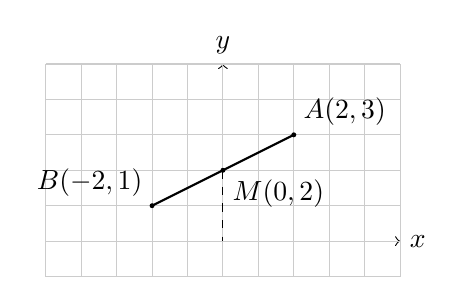
\begin{tikzpicture}[scale=0.45]
	\draw[->] (-5,0)--(5,0) node[right] {$x$};
	\draw[->] (0,-1)--(0,5) node[above] {$y$};
	\draw[gray!40] (-5,-1) grid[step=1] (5,5);
	\fill (2,3) circle (2pt) node[above right] {$A(2,3)$};
	\fill (-2,1) circle (2pt) node[above left] {$B(-2,1)$};
	\fill (0,2) circle (2pt) node[below right] {$M(0,2)$};
	\draw[thick] (-2,1)--(2,3);
	\draw[dashed] (0,2)--(0,0);
\end{tikzpicture}
\end{center}

\newpage
\section{2点間の距離 解答}
\begin{align*}
&1.\ 2\sqrt{5}\\
&2.\ 2\sqrt{34}\\
&3.\ 8\sqrt{2}\\
&4.\ 7\\
&5.\ \sqrt{29}\\
&6.\ \frac{2\sqrt{65}}{3}\\
&7.\ \frac{2\sqrt{97}}{3}\\
&8.\ \frac{3}{2}
\end{align*}
\textbf{考え方}\
距離は $\sqrt{(x_2-x_1)^2+(y_2-y_1)^2}$。中点間距離は先に中点を出して同じ式に代入。\\
\textbf{途中式（代表例）}
\begin{align*}
&1.\ AB=\sqrt{(-2-2)^2+(1-3)^2}=\sqrt{16+4}=2\sqrt5\\
&4.\ M_{AB}=(0,2),\ M_{CD}=(0,-5)\Rightarrow d=\sqrt{0^2+(-7)^2}=7\\
&6.\ M_{ABC}=\left(\frac43,-\frac53\right),\ D=(-4,-1)\\
&\quad d=\sqrt{\left(-4-\frac43\right)^2+\left(-1+\frac53\right)^2}=\sqrt{\frac{260}{9}}=\frac{2\sqrt{65}}{3}
\end{align*}
\textbf{図説（距離公式）}
\begin{center}
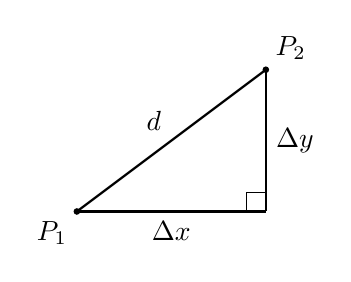
\begin{tikzpicture}[scale=0.6]
	\coordinate (A) at (0,0);
	\coordinate (B) at (4,3);
	\coordinate (C) at (4,0);
	\draw[thick] (A)--(B) node[midway,above left] {$d$};
	\draw[thick] (A)--(C) node[midway,below] {$\Delta x$};
	\draw[thick] (C)--(B) node[midway,right] {$\Delta y$};
	\draw (3.6,0) -- (3.6,0.4) -- (4,0.4);
	\fill (A) circle (2pt) node[below left] {$P_1$};
	\fill (B) circle (2pt) node[above right] {$P_2$};
\end{tikzpicture}
\end{center}

\newpage
\section{2点間の移動 解答}
(1秒あたりの移動量)
\begin{align*}
&1.\ (-2,-1)\\
&2.\ \left(\frac{1}{2},-3\right)\\
&3.\ (-3,-2)\\
&4.\ \left(\frac{3}{2},-\frac{5}{2}\right)\\
&5.\ (-1,-1)\\
&6.\ (-2,2)\\
&7.\ (2,1)\\
&8.\ \left(-\frac{1}{2},3\right)
\end{align*}
\textbf{考え方}\
1秒あたり移動量は「終点−始点」を秒数で割る。\\
\textbf{途中式（代表例）}
\begin{align*}
&1.\ \Delta=((-2)-2,\ 1-3)=(-4,-2),\ \frac{\Delta}{2}=(-2,-1)\\
&4.\ \Delta=(4-(-2),\ -9-1)=(6,-10),\ \frac{\Delta}{4}=\left(\frac32,-\frac52\right)\\
&8.\ \Delta=(2-4,\ 3-(-9))=(-2,12),\ \frac{\Delta}{4}=\left(-\frac12,3\right)
\end{align*}

\newpage
\section{円の当たり判定1 解答}
\begin{align*}
&1.\ |AB|=\sqrt{45}=3\sqrt{5}>1+2=3\ \Rightarrow\ \text{当たらない}\\
&2.\ |AC|=\sqrt{2}<1+3=4\ \Rightarrow\ \text{当たる。必要移動量}=4-\sqrt{2}
\end{align*}
\textbf{考え方}\
中心間距離 $d$ と半径和 $r+R$ を比較し、$d\le r+R$ なら接触。めり込み量は $(r+R)-d$。\\
\textbf{途中式（代表例）}
\begin{align*}
&1.\ d_{AB}=\sqrt{(4-1)^2+(8-2)^2}=\sqrt{45}>3\Rightarrow\text{非接触}\\
&2.\ d_{AC}=\sqrt{(0-1)^2+(1-2)^2}=\sqrt2<4\Rightarrow\text{接触, めり込み}=4-\sqrt2
\end{align*}
\textbf{図説（円同士の判定）}
\begin{center}
\begin{tikzpicture}[scale=0.5]
	\draw (0,0) circle (1.2);
	\draw (4,0) circle (1.8);
	\fill (0,0) circle (2pt) node[below] {$O_1$};
	\fill (4,0) circle (2pt) node[below] {$O_2$};
	\draw[<->] (0,0.2)--(4,0.2) node[midway,above] {$d$};
	\node at (0,1.7) {$r$};
	\node at (4,2.3) {$R$};
	\node at (2,-1.8) {$d\le r+R\Rightarrow\text{接触}$};
\end{tikzpicture}
\end{center}

\newpage
\section{円の当たり判定2 解答}
\begin{align*}
&1.\ \text{Aの必要総移動}=4\ \Rightarrow\ 1\text{秒あたり }(2,0)\\
&2.\ \text{Bの必要総移動}=4\ \Rightarrow\ 1\text{秒あたり }(1,0)
\end{align*}
\textbf{考え方}\
接触条件は中心間距離が半径和になること。必要総移動量を時間で割る。\\
\textbf{途中式（代表例）}
\begin{align*}
&1.\ A(0,0),B(7,0),\ r+R=3\Rightarrow \text{必要距離}=7-3=4,\ 2\text{秒} \Rightarrow (2,0)\\
&2.\ B(7,0),C(16,0),\ r+R=5\Rightarrow \text{必要距離}=16-7-5=4,\ 4\text{秒} \Rightarrow (1,0)
\end{align*}

\newpage
\section{円の当たり判定の一般化 解答}
\begin{align*}
&1.\ \sqrt{(a-c)^2+(b-d)^2}\le r+R\\
&2.\ (a-c)^2+(b-d)^2\le (r+R)^2
\end{align*}
\textbf{考え方}\
一般点でも同じく中心間距離と半径和を比較する。2乗して根号を外す。\\
\textbf{途中式（代表例）}
\begin{align*}
d&=\sqrt{(a-c)^2+(b-d)^2},\ \text{接触条件 }d\le r+R\\
\Rightarrow\ &(a-c)^2+(b-d)^2\le (r+R)^2
\end{align*}
\end{document}


